% !TeX program = xelatex
% A题程序运行与结果说明（竞赛交付技术简报）
% 指标由 report_metrics.csv 经 report_metrics.tex 自动注入，禁止手工改写数值。
\documentclass[UTF8,a4paper,zihao=-4]{ctexart}

\usepackage[margin=18mm]{geometry}
\usepackage{fontspec}
\usepackage{graphicx}
\usepackage{booktabs}
\usepackage{tabularx}
\usepackage{xcolor}
\usepackage{tcolorbox}
\usepackage{enumitem}
\usepackage{hyperref}
\usepackage{microtype}
\usepackage{caption}
\usepackage{float}

\definecolor{MainBlue}{HTML}{2F6F9F}
\definecolor{WarnOrange}{HTML}{D97732}
\definecolor{NeutralGray}{HTML}{5B6470}

\hypersetup{
  colorlinks=true,
  linkcolor=MainBlue,
  urlcolor=MainBlue,
  citecolor=MainBlue,
  pdftitle={A题 世界杯比赛数据挖掘与预测——程序运行与结果说明},
  pdfauthor={APMCM Problem A}
}

\tcbuselibrary{skins,breakable}
\tcbset{
  colback=white,
  colframe=MainBlue,
  boxrule=0.7pt,
  arc=0.8pt,
  left=6pt,right=6pt,top=5pt,bottom=5pt,
  fonttitle=\bfseries
}

\captionsetup{font=small,labelfont={bf,color=MainBlue},skip=4pt}
\setlist[itemize]{leftmargin=1.4em,itemsep=1.5pt,topsep=2pt}
\setlist[enumerate]{leftmargin=1.5em,itemsep=1.5pt,topsep=2pt}
\setlength{\parskip}{0.35em}
\setlength{\parindent}{0pt}

% Auto-generated from outputs/report_metrics.csv — do not edit.
\makeatletter
\newcommand{\MetricDataMinYear}{1930}
\newcommand{\MetricDataMaxYear}{2014}
\newcommand{\MetricTournamentCount}{20}
\newcommand{\MetricMatchCount}{836}
\newcommand{\MetricPOneRTwo}{0.792}
\newcommand{\MetricPOneAdjRTwo}{0.753}
\newcommand{\MetricPOnePredTwentyEighteen}{160.10}
\newcommand{\MetricPOneActualTwentyEighteen}{169}
\newcommand{\MetricPOneMaxVif}{18.44}
\newcommand{\MetricPTwoPearson}{0.696}
\newcommand{\MetricPTwoMae}{0.984}
\newcommand{\MetricPTwoMse}{1.388}
\newcommand{\MetricPTwoRTwo}{0.547}
\newcommand{\MetricPThreeModel}{题面四特征多分类逻辑回归}
\newcommand{\MetricPThreeC}{0.001}
\newcommand{\MetricPThreeAcc}{0.578125}
\newcommand{\MetricPThreeAccShort}{0.578}
\newcommand{\MetricPThreeCorrect}{37}
\newcommand{\MetricPThreeN}{64}
\newcommand{\MetricPThreeMacroFOne}{0.465}
\newcommand{\MetricPThreeDrawRecall}{0.077}
\makeatother


\title{\vspace{-1.2em}\bfseries\textcolor{MainBlue}{A题 世界杯比赛数据挖掘与预测\\——程序运行与结果说明}}
\author{程序运行技术说明（指标源：\texttt{outputs/report\_metrics.csv}）}
\date{}

\begin{document}
\maketitle
\vspace{-1.2em}

\begin{tcolorbox}[title=运行与提交协议]
\begin{tabularx}{\textwidth}{@{}lX@{}}
\toprule
\textbf{项目} & \textbf{规定} \\
\midrule
Python 版本 & 3.8 \\
程序入口 & \texttt{python3 main.py}（默认执行六问分析并生成预测文件） \\
测试数据目录 & \texttt{/testdata}；亦可由 \texttt{--testdata} 或环境变量 \texttt{TESTDATA\_DIR} 指定 \\
预测输出文件 & 源码目录下的 \texttt{./cla\_pre.csv} \\
类别编码 & \texttt{prediction}$\,\in\,\{0,1,2\}$，依次表示主胜、平局、客胜 \\
行序约束 & 输出行与查询输入行按位置一一对应，不得按编号重排 \\
六问产物 & 自动写入 \texttt{outputs/tables}、\texttt{outputs/figures}、\texttt{outputs/logs} 及指标源 CSV \\
\bottomrule
\end{tabularx}
\end{tcolorbox}

\subsection*{主要结果摘要}
\begin{itemize}
  \item 样本范围：\MetricDataMinYear--\MetricDataMaxYear，共 \MetricTournamentCount\ 届、\MetricMatchCount\ 场比赛。
  \item 第2问（2018 总进球回归）：三特征线性模型预测值为 \MetricPOnePredTwentyEighteen，对应实际值为 \MetricPOneActualTwentyEighteen；拟合优度 $R^2=\MetricPOneRTwo$。
  \item 第6问（2014 测试）：模型为\MetricPThreeModel；正确分类 \MetricPThreeCorrect/\MetricPThreeN 场，准确率为 \MetricPThreeAcc。
\end{itemize}

\section{程序结构与六问对应关系}
核心文件包括：\texttt{main.py}（正式入口）、\texttt{analyze.py}（仅分析）、\texttt{problem1\_analysis.py}、\texttt{problem2\_analysis.py}、\texttt{problem3\_analysis.py}、\texttt{prediction\_api.py} 与 \texttt{report\_data.py}。

{\footnotesize
\noindent
\begin{tabular}{@{}c p{4.2cm} p{9.0cm}@{}}
\toprule
\textbf{问} & \textbf{实现脚本} & \textbf{自动生成结果} \\
\midrule
1 & \texttt{problem1\_analysis.py} & 四项描述统计、图1与图2、文字结论 \\
2 & \texttt{problem1\_analysis.py} & 2018 线性回归口径及预测表 \\
3 & \texttt{problem2\_analysis.py} & 阶段进球统计、半场--全场相关及图4 \\
4 & \texttt{problem2\_analysis.py} & 2014 单场进球基准 MAE/MSE/$R^2$ 与可复用接口 \\
5 & \texttt{problem3\_analysis.py} & 四特征及相关诊断（Spearman、VIF、结局指示变量）与图5 \\
6 & \texttt{problem3\_analysis.py} & 2014 逻辑回归指标、混淆矩阵（图6）及 2026 预测接口 \\
\bottomrule
\end{tabular}
\par
}

\noindent\textbf{处理流程。}
\texttt{/testdata}（或打包目录 \texttt{data/}）
$\rightarrow$ 数据读取与校验
$\rightarrow$ 六问统计分析与模型拟合
$\rightarrow$ 写入 \texttt{outputs/}（表、图、日志）及 \texttt{report\_metrics.csv}
$\rightarrow$ 查询预测
$\rightarrow$ 输出 \texttt{cla\_pre.csv}。

\section{问题一与问题二的程序输出}
\textbf{问题一。}
程序对世界杯汇总表计算总进球、场均进球、参赛队数与比赛场次四项描述统计；生成总进球相对赛会规模的双轴趋势图及场均进球趋势图；并以参赛队数、比赛场次、观众数三特征建立线性回归，复现 2018 年总进球。

\textbf{数值结果。}
2018 年预测值为 \MetricPOnePredTwentyEighteen，实际值为 \MetricPOneActualTwentyEighteen；
$R^2=\MetricPOneRTwo$，调整 $R^2=\MetricPOneAdjRTwo$，最大 VIF 为 \MetricPOneMaxVif。
在多重共线性较强时，单系数不宜解释为独立边际效应；该模型仅用于总体预测。

\begin{figure}[H]
\centering
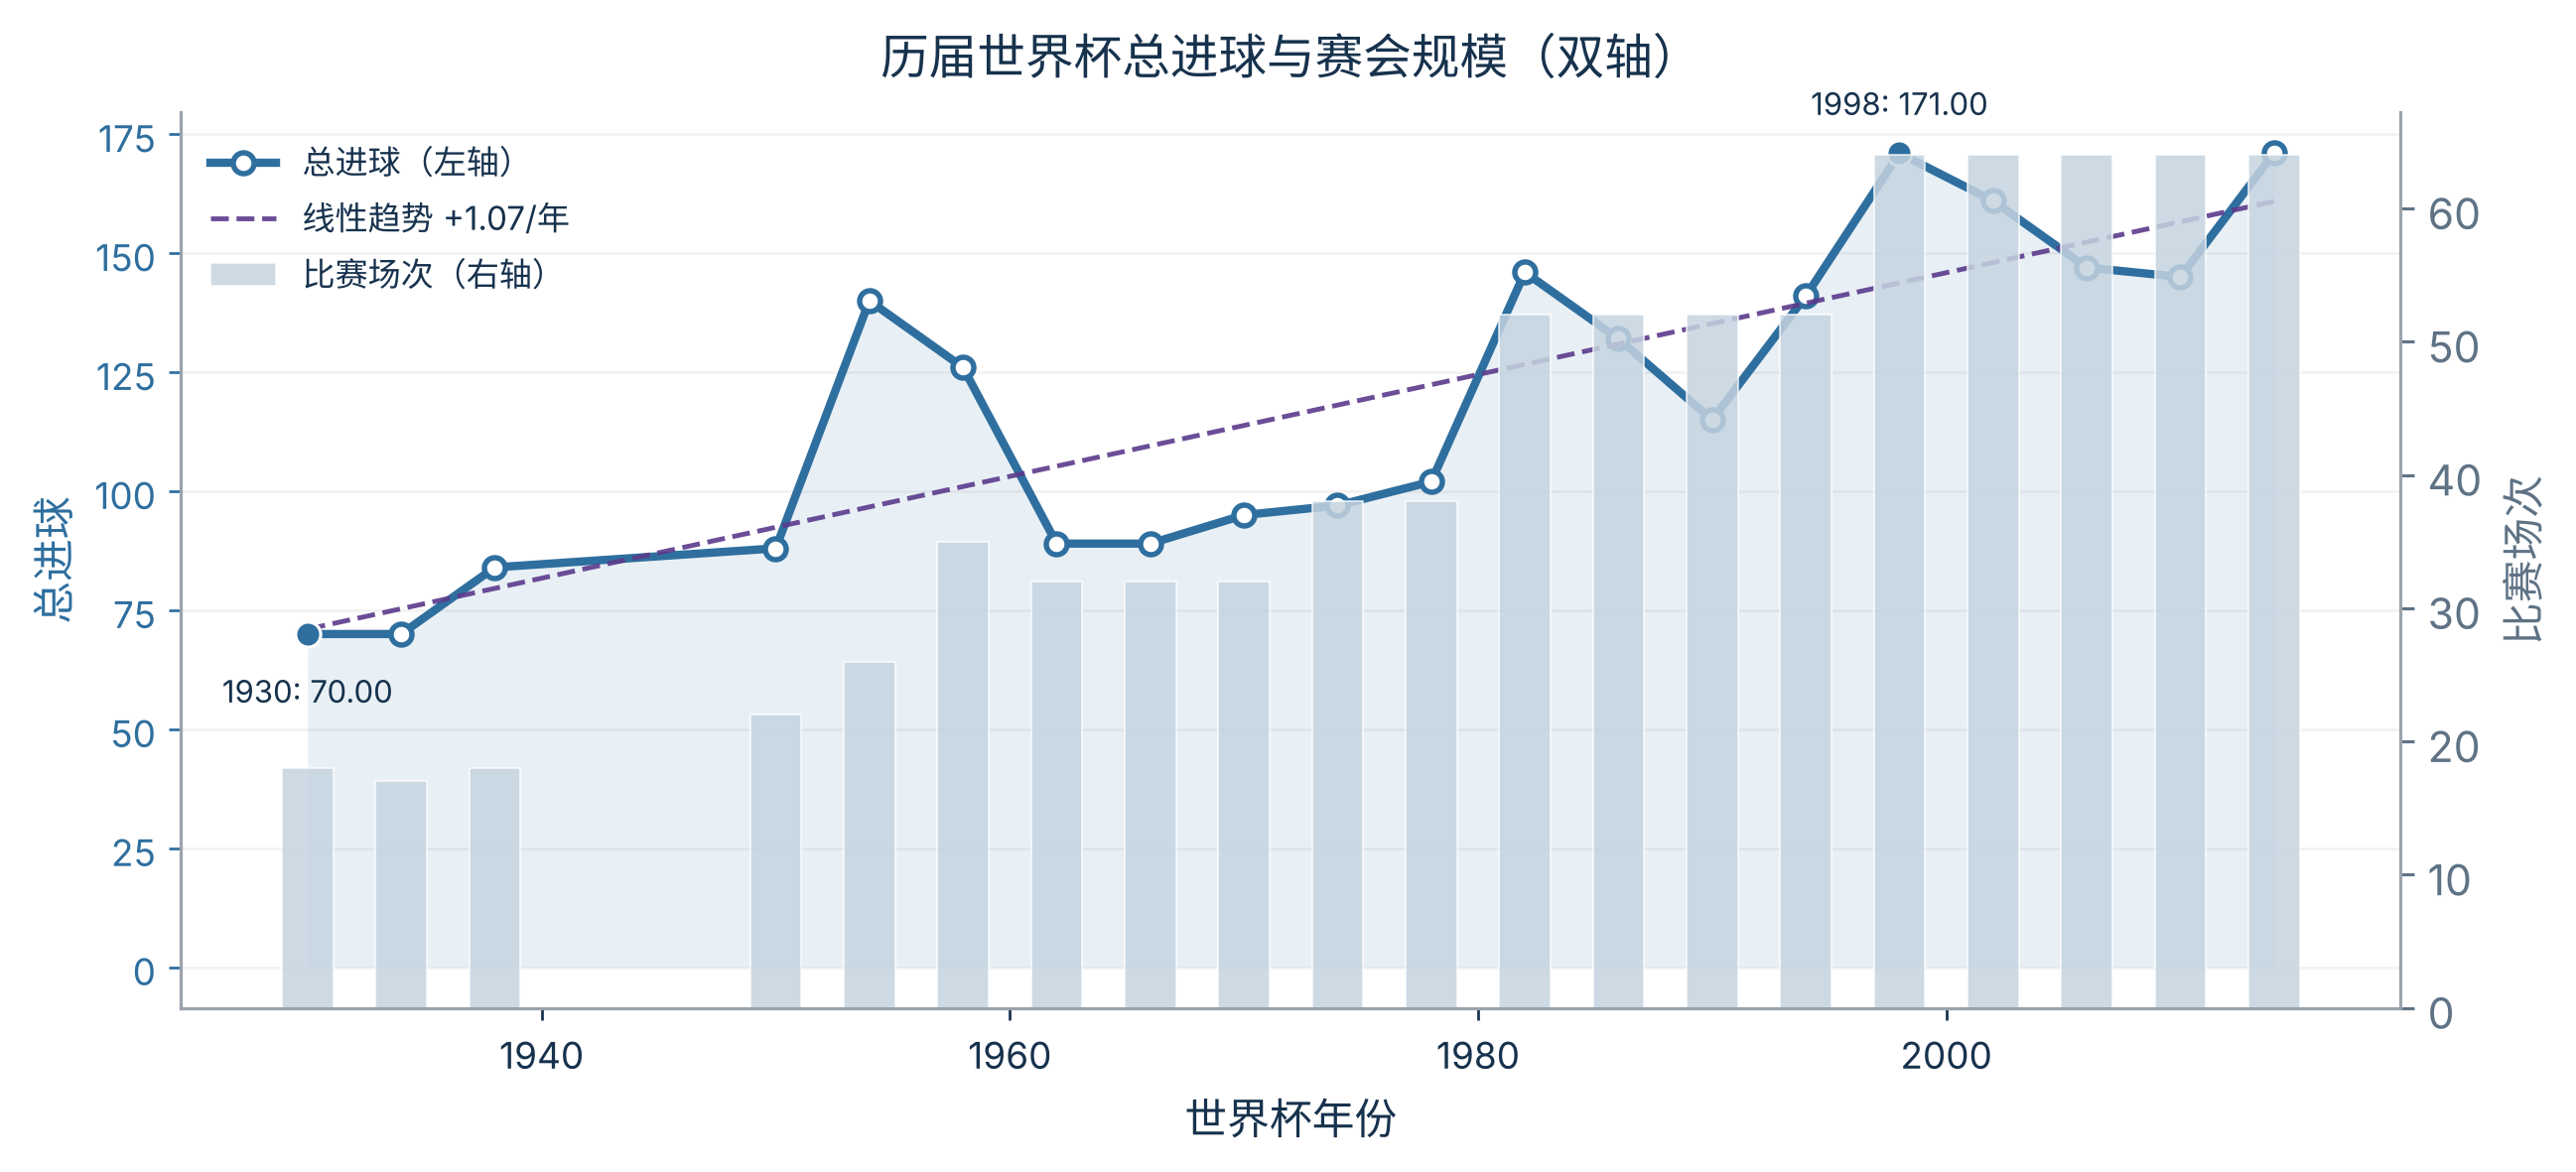
\includegraphics[width=0.92\textwidth]{../outputs/figures/图1_总进球趋势.png}
\caption{历届总进球与比赛场次的双轴对照：总量上升与赛会规模扩张同步出现。}
\end{figure}

\textbf{问题二。}
程序按比赛阶段汇总场均总进球；计算半场总进球与全场总进球的 Pearson 相关系数；实现题面规定的单场总进球线性回归，并在 2014 年历史开发基准上报告误差指标。

\textbf{数值结果。}
半场与全场总进球的 Pearson 相关系数为 $r=\MetricPTwoPearson$；
2014 年题面单场模型的 MAE、MSE 与 $R^2$ 分别为 \MetricPTwoMae、\MetricPTwoMse 与 \MetricPTwoRTwo。

\begin{figure}[H]
\centering
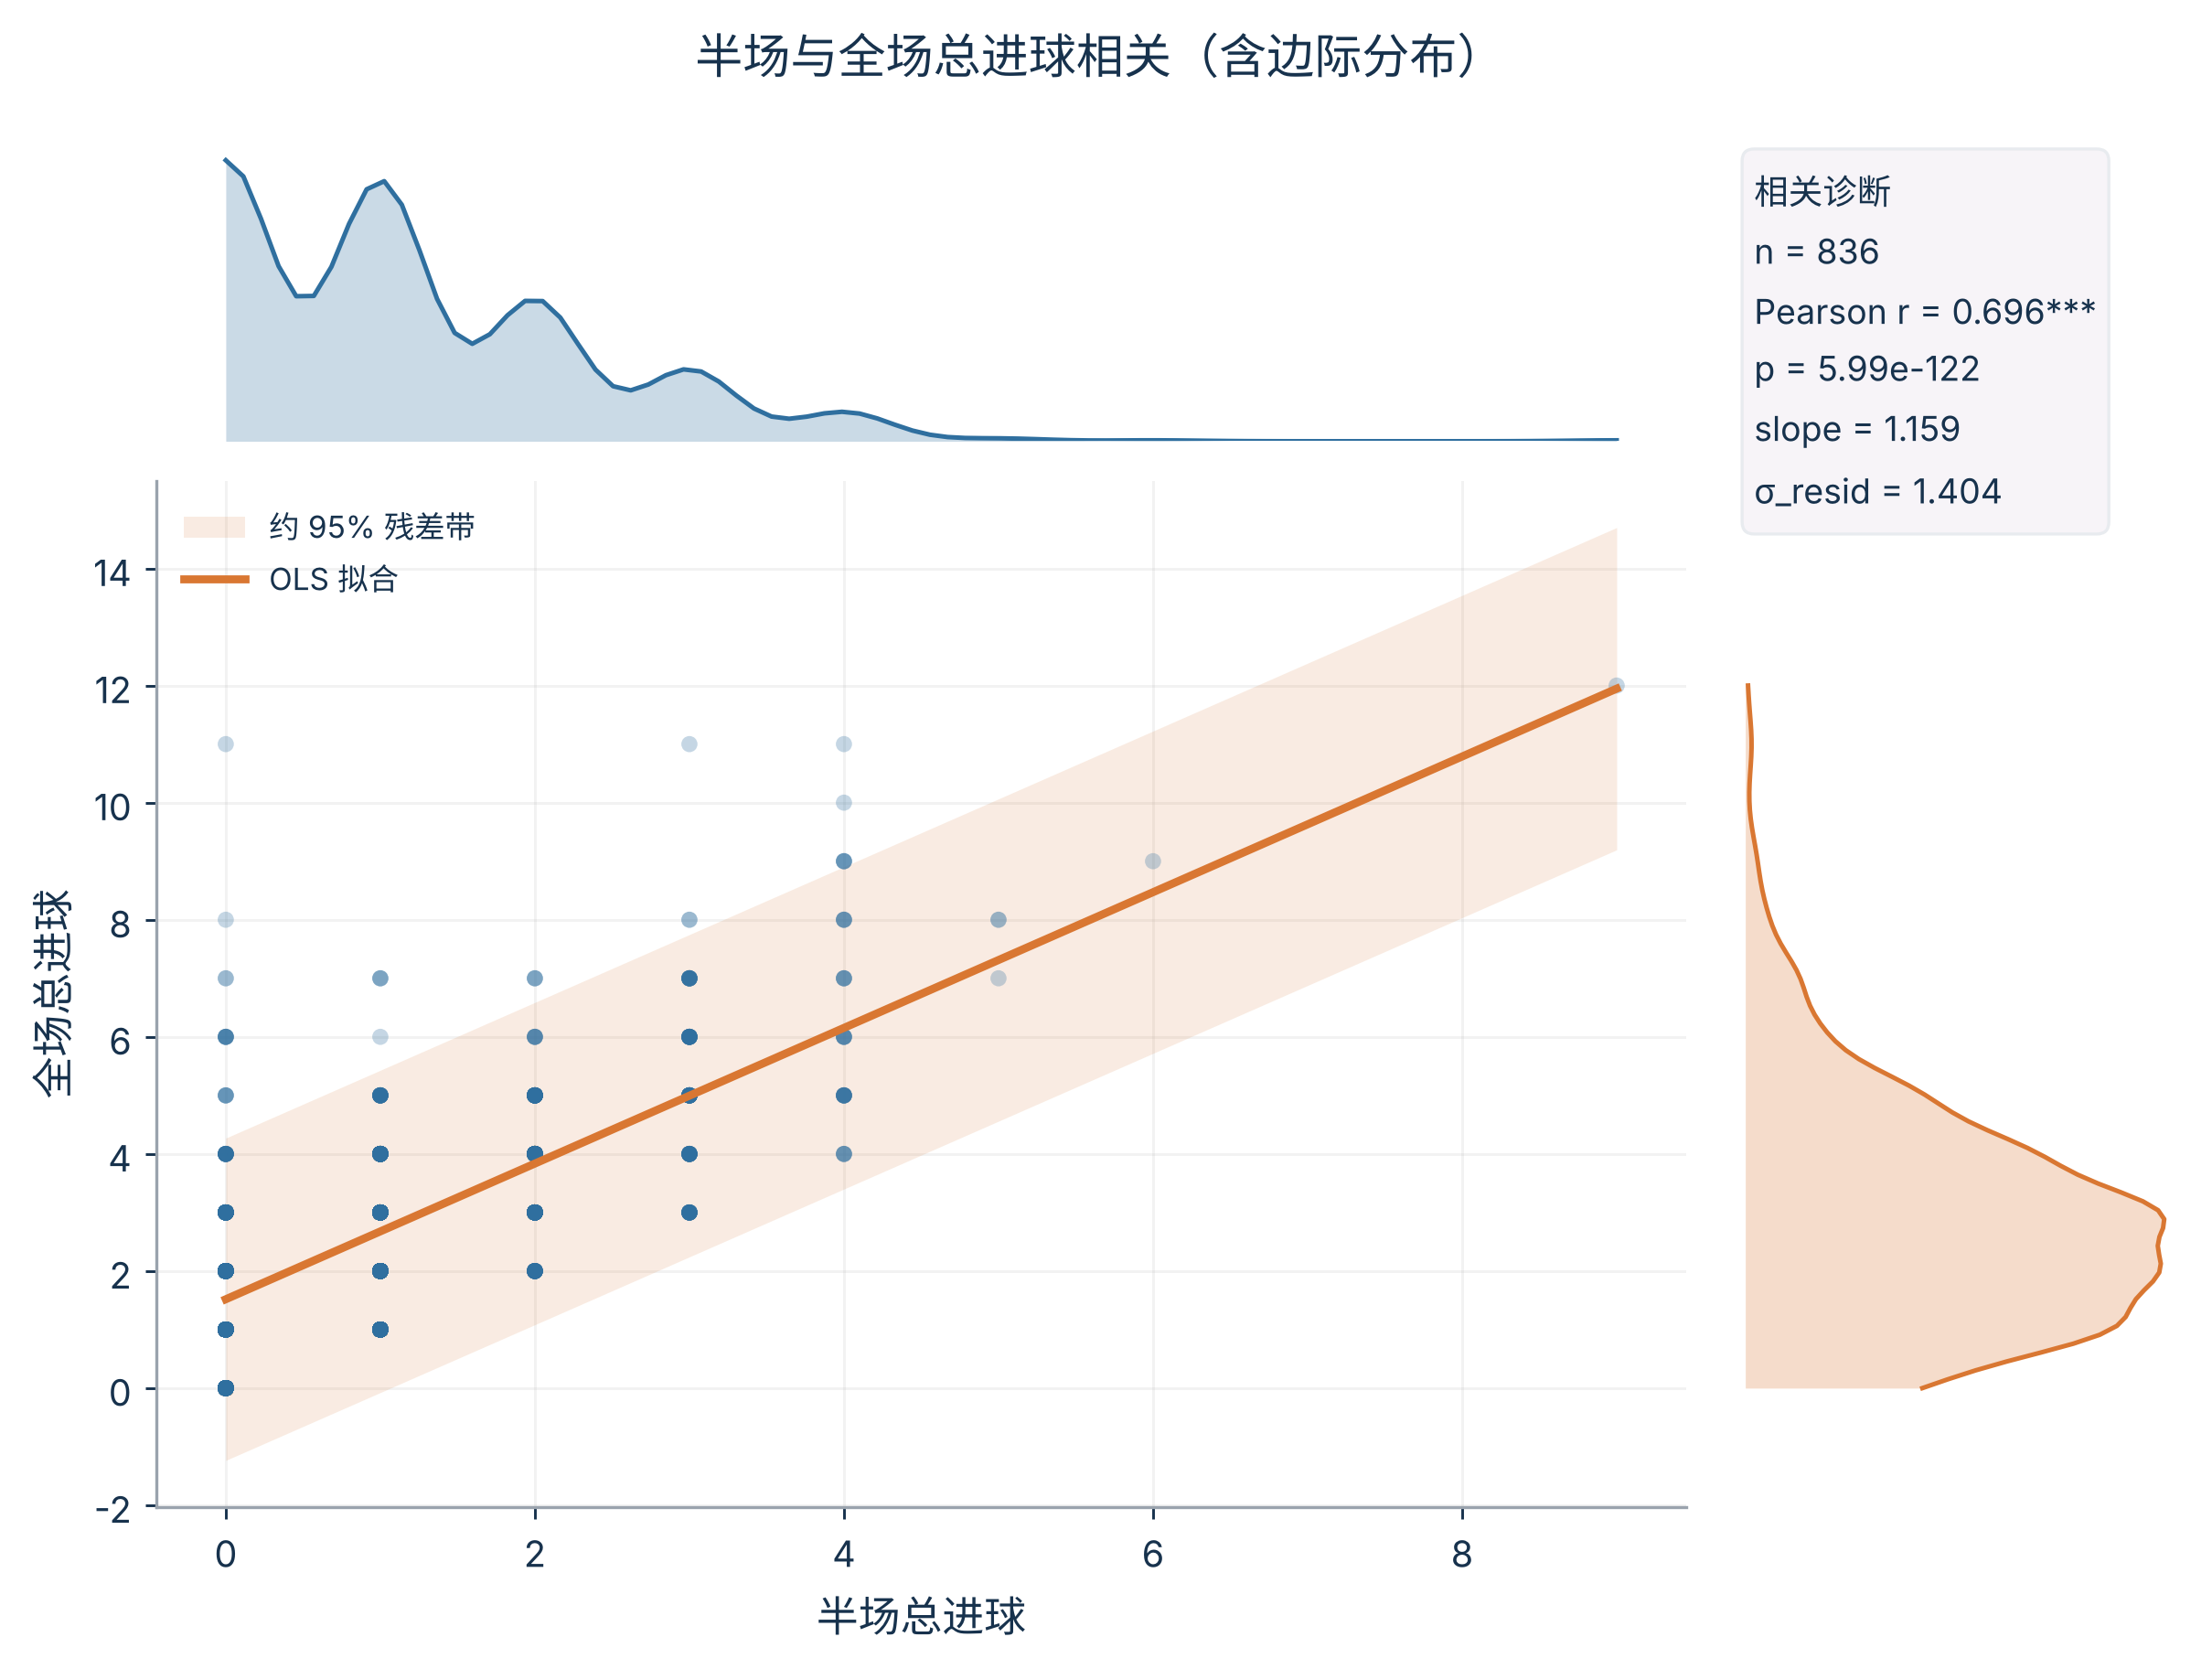
\includegraphics[width=0.78\textwidth]{../outputs/figures/图4_半场与全场进球相关.png}
\caption{半场总进球与全场总进球的散点、OLS 拟合及边际分布；$r=\MetricPTwoPearson$。}
\end{figure}

\section{问题三：逻辑回归、2014 测试与 2026 接口}
\textbf{模型设定。}
正式模型为题面规定的四特征多分类逻辑回归，特征为主客队在参赛次数、最佳成绩、场均进球与场均失球上的差值。
训练区间为 1930--2010；2014 为固定测试集，不作盲测表述。
正则化参数 $C=\MetricPThreeC$，类别权重取 \texttt{balanced}；超参数仅在 2014 年之前的滚动验证折上选定。

\textbf{2014 测试结果。}
正确分类 \MetricPThreeCorrect/\MetricPThreeN 场，准确率为 \MetricPThreeAcc；
Macro-F1 为 \MetricPThreeMacroFOne；平局类别召回率为 \MetricPThreeDrawRecall。

\begin{figure}[H]
\centering
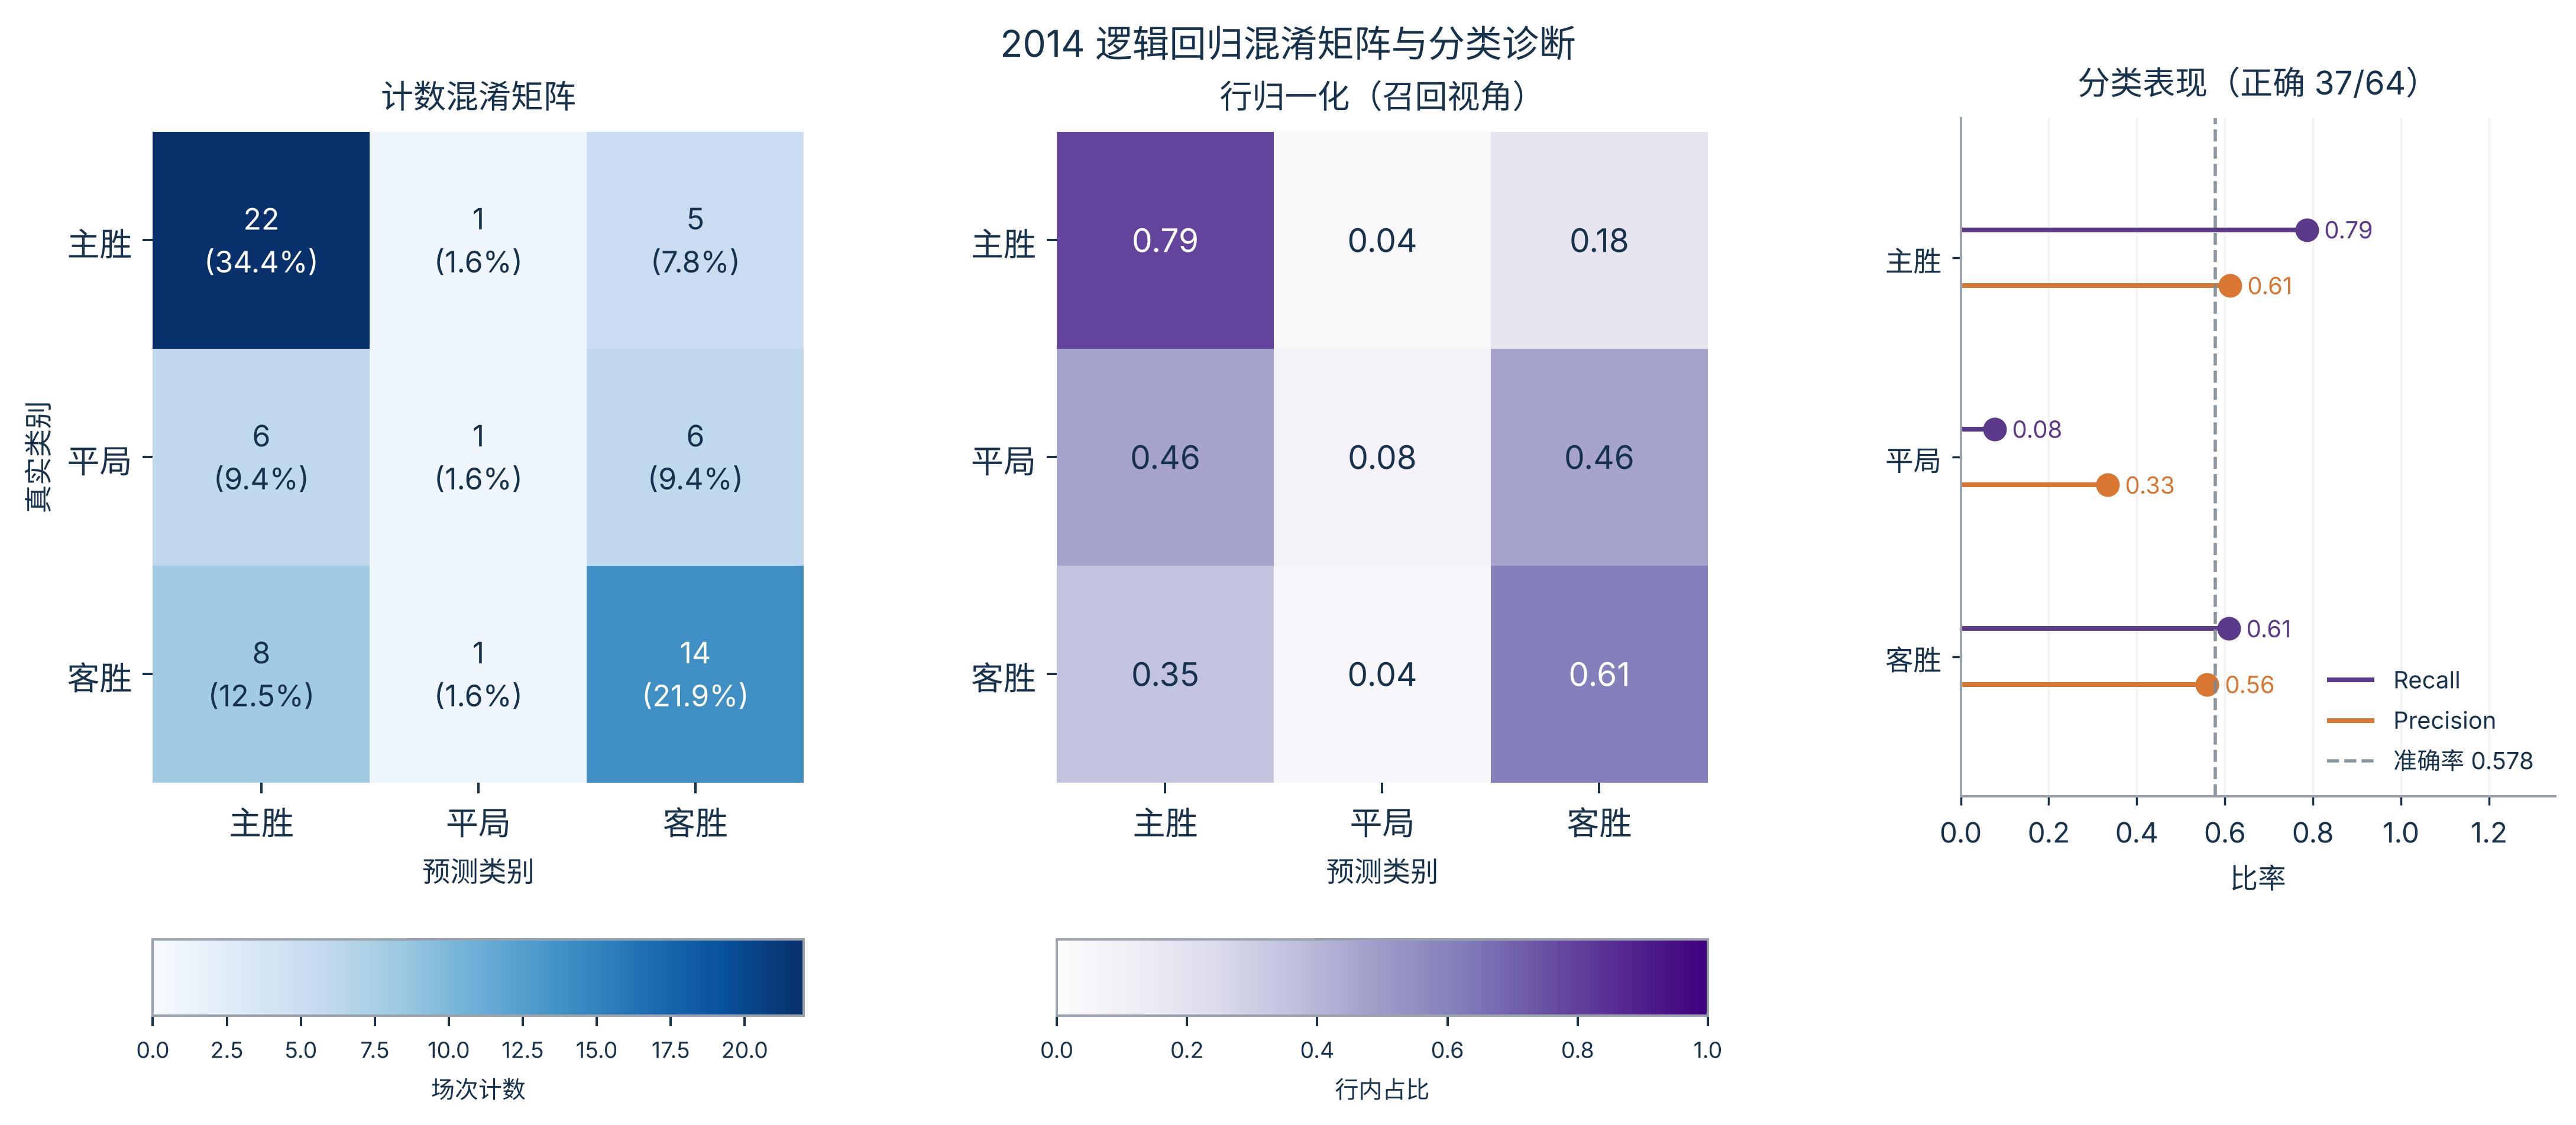
\includegraphics[width=0.96\textwidth]{../outputs/figures/图6_2014逻辑回归混淆矩阵.png}
\caption{2014 测试集混淆矩阵：计数分布、行归一化召回及各类 Precision/Recall。}
\end{figure}

\begin{figure}[H]
\centering
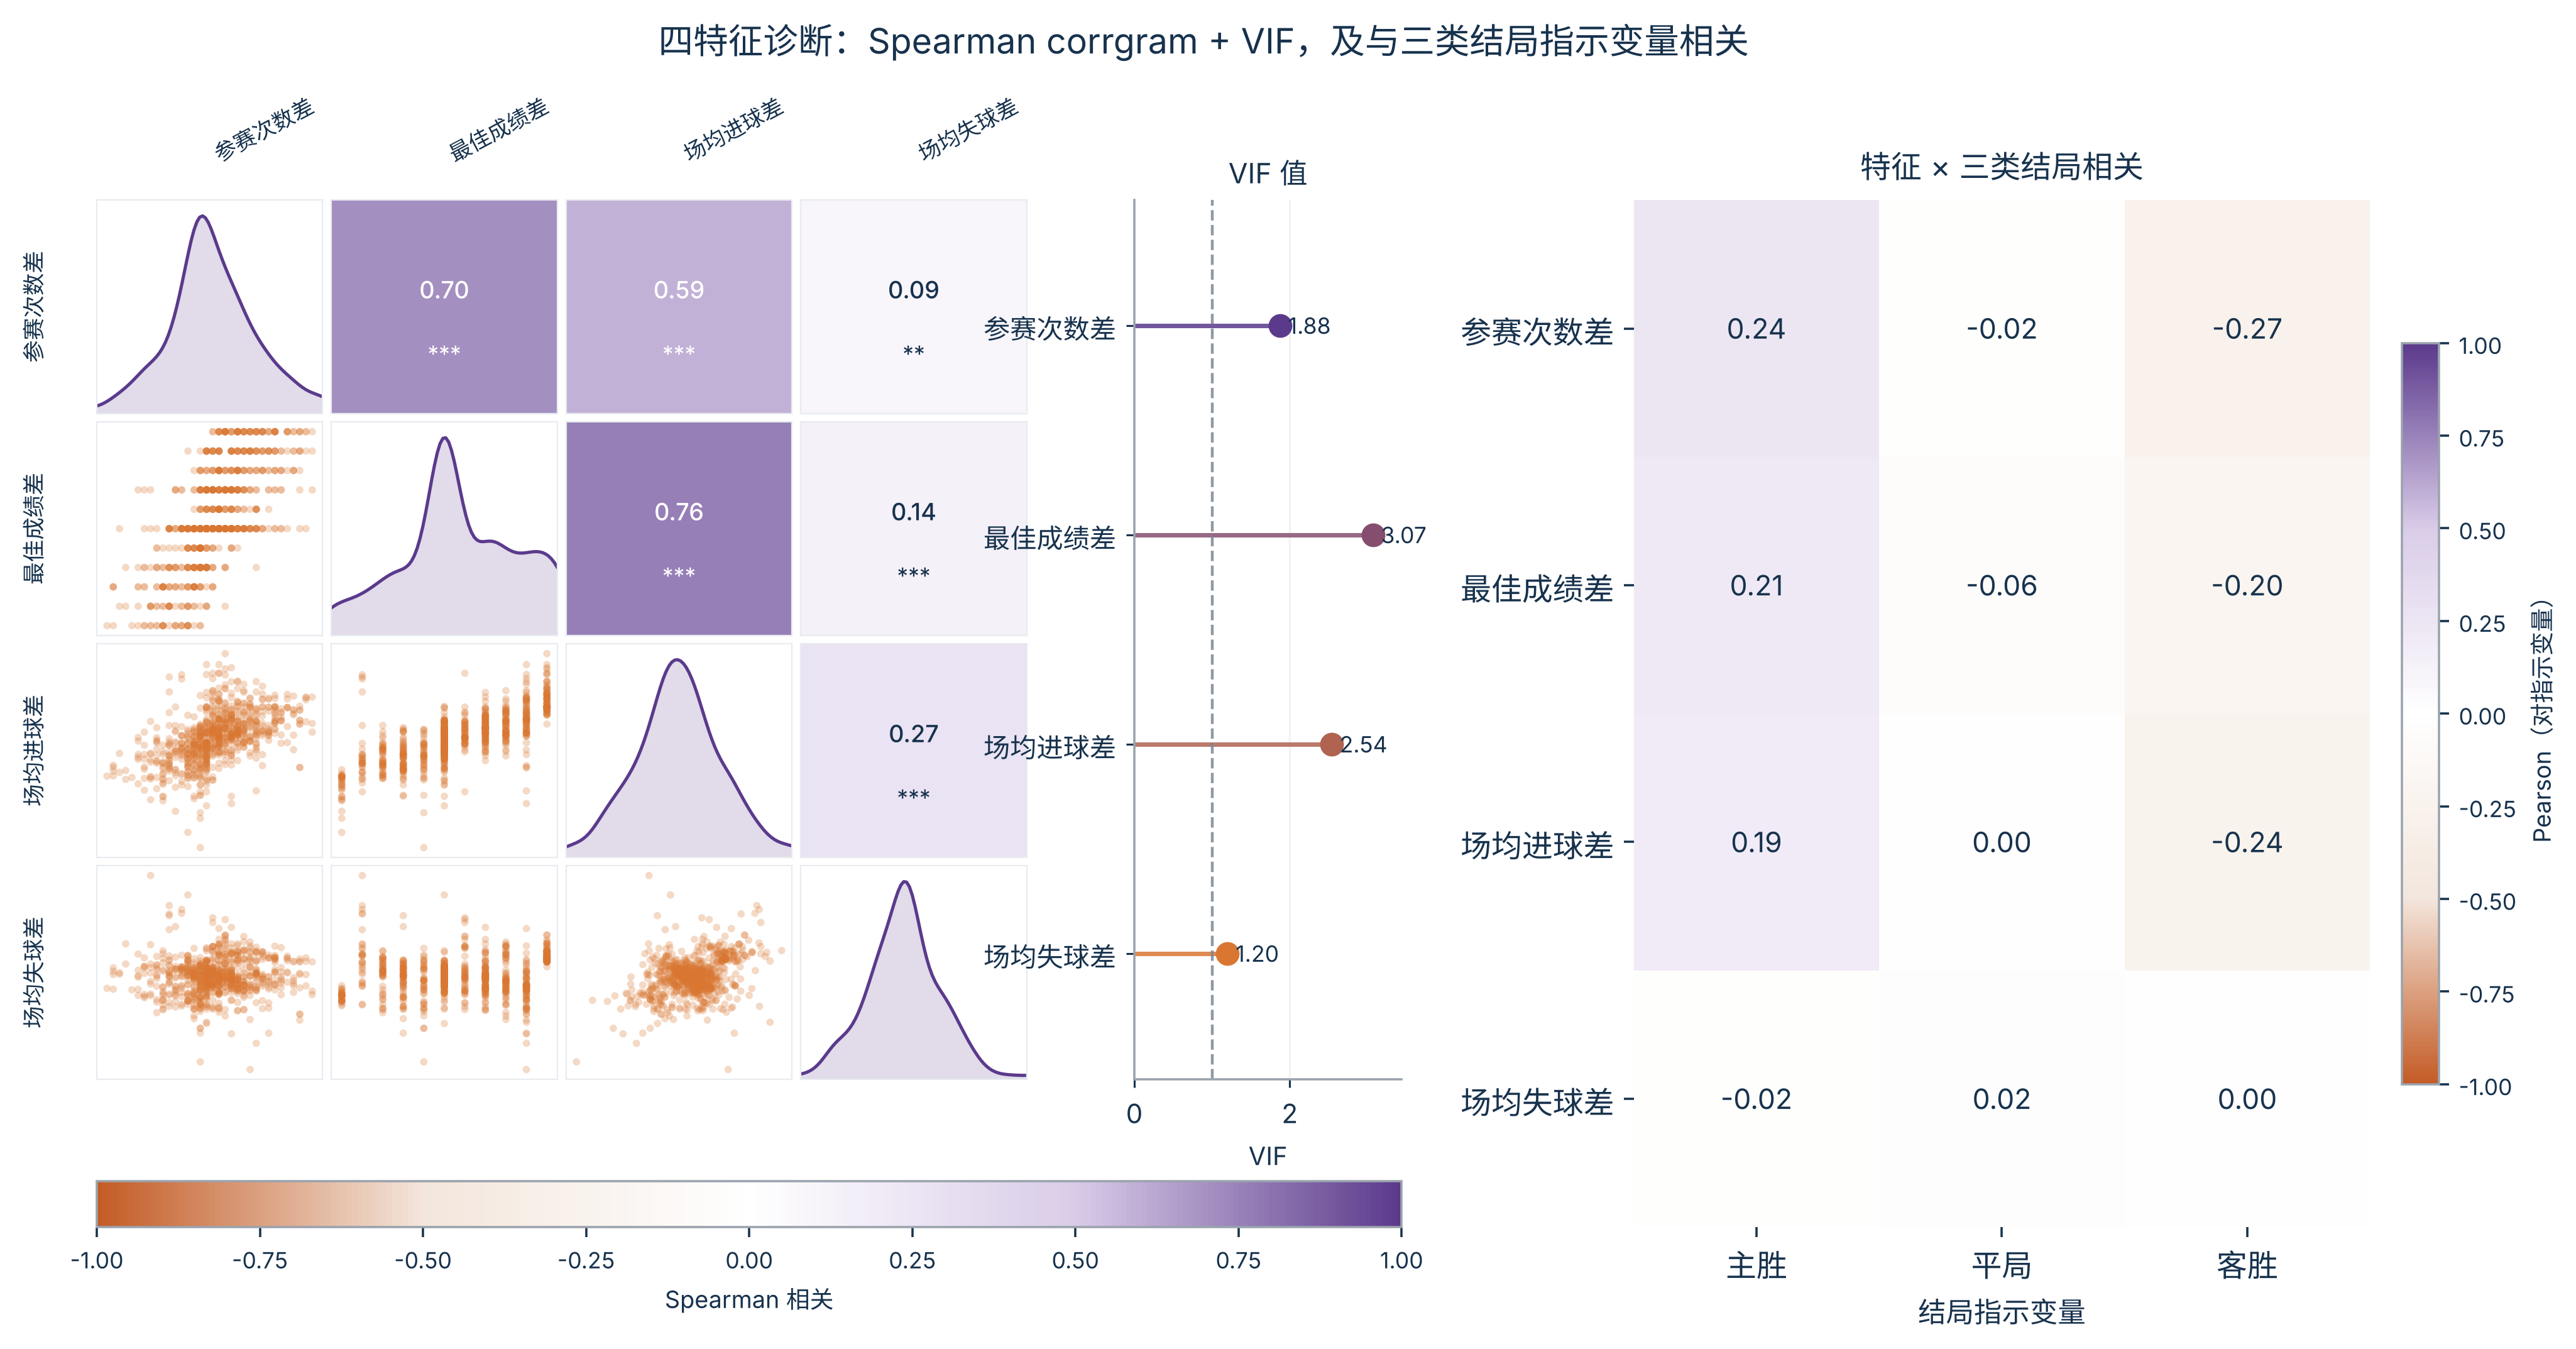
\includegraphics[width=0.96\textwidth]{../outputs/figures/图5_问题三四特征相关热力图.png}
\caption{四特征 Spearman 相关与 VIF；结局相关按主胜、平局、客胜指示变量分别计算。}
\end{figure}

\textbf{\texttt{cla\_pre.csv} 协议。}
\begin{itemize}
  \item 查询输入可为单独的 \texttt{query.csv}，或比赛表中主客队进球缺失的嵌入行；二者不得同时出现。
  \item 存在有效编号时输出列为 \texttt{id,prediction}；否则仅输出 \texttt{prediction}。
  \item 硬分类标签与三类概率的 argmax 保持一致；文件采用 UTF-8-BOM，并以原子替换方式写入。
  \item 未知球队触发警告后，采用中性先验特征，仍返回有限数值预测。
  \item 缺少主客队字段，或正式模式下不存在任何查询记录时，程序以非零状态退出；不得自动切换至演示输入。
\end{itemize}

\section{依赖、运行步骤、输出目录与复现}
\subsection*{环境依赖}
运行环境为 Python 3.8。依赖见 \texttt{requirements.txt}（NumPy、pandas、SciPy、scikit-learn、Matplotlib）。
安装命令：\texttt{python -m pip install -r requirements.txt}。本说明文档由 XeLaTeX 编译。

\subsection*{运行命令}
\begin{verbatim}
python3 main.py
python3 main.py --demo --details
python3 main.py --testdata <目录>
python release_check.py
cd doc && python build_latex.py
\end{verbatim}
\texttt{analyze.py} 仅用于单独重算分析产物；正式提交与判题入口为 \texttt{main.py}。

\subsection*{输出目录}
\begin{itemize}
  \item \texttt{cla\_pre.csv}：预测提交文件（位于源码根目录）
  \item \texttt{outputs/tables/}：统计表与模型指标
  \item \texttt{outputs/figures/}：规定图件
  \item \texttt{outputs/logs/}：文字结论
  \item \texttt{outputs/report\_metrics.csv}：说明文档唯一指标源
\end{itemize}

\subsection*{异常行为}
缺少依赖时抛出 \texttt{ModuleNotFoundError}；缺少查询数据时失败退出。出现多份 \texttt{query.csv}、字段非法，或查询文件与嵌入查询行并存时，程序终止并返回非零退出码。

\subsection*{复现核对}
\begin{enumerate}
  \item 在干净目录解压 \texttt{src}，安装依赖后执行 \texttt{python3 main.py --demo}。
  \item 确认生成 \texttt{cla\_pre.csv} 与 \texttt{outputs/} 目录。
  \item 核对 PDF 中数值与 \texttt{report\_metrics.csv} 一致。
  \item 执行 \texttt{python release\_check.py}，全部检查项通过。
\end{enumerate}

\end{document}
